\documentclass{beamer}
\newcommand{\myfont}{\rmfamily\normalsize\upshape\mdseries}
\newcommand{\degree}{^\circ}
\title{\sffamily Review VIII(Slides 418 - 486)}
\subtitle{\textbf{Graph Theory}\\Construct your graph in a nice way!}
\institute[UM-SJTU JI]{University of Michigan-Shanghai Jiao Tong University Joint Institute}
\author{HamHam}
\usepackage{graphicx}
\usepackage{picinpar}
\usepackage{indentfirst}
\usepackage{chemformula}
\usepackage{geometry}
\usepackage{subfigure}
\usepackage{appendix}
\usepackage{amsfonts}
\usepackage{enumerate}
\usepackage{float}
\usepackage{geometry}
\usepackage{latexsym}
\usepackage{listings}
\usepackage{multicol,multirow,multido}
\usepackage{tabularx}
\usepackage{ulem}
\usepackage{tikz}
\usepackage{xcolor}
\usepackage{cite}
\usepackage{setspace}
\usepackage{hyperref}
\usepackage{textpos}
\usepackage{booktabs}
\usepackage{diagbox}
\usepackage{listings}
\usepackage{graphics}
\usepackage{upgreek}
\usepackage{JI_MathCourse_Notations}
\usepackage{mathrsfs}


%\usepackage{ctex} %插入中文
%\ctexset{today=old}

\newcommand{\mydef}[1]{\sffamily\blue{#1}\myfont\\} %for define
\newcommand{\mysol}{\yellow{Solution:}\\}
\usetheme[dove]{Boadilla}
\usecolortheme{dolphin}
\useoutertheme{miniframes}
\begin{document}
    \usebackgroundtemplate{\tikz\node[opacity=0.25]{
    
\includegraphics[width=\paperwidth,
    height=\paperheight]{hamster.jpg}
    };}
\begin{titlepage}
    \begin{center}
        VE203 - Discrete Mathmatics 
    \end{center}
\end{titlepage}
\myfont
\newcommand{\binomial}[2]{\begin{pmatrix} {#1}\\{#2}	\end{pmatrix}}
\newcommand{\green}[1]{\textcolor[rgb]{0.3,0.6,0}{#1}}
\section{Asymptotic Notation}
\begin{frame}
    \frametitle{Asymptotic Notation}
    We define: 
    \begin{equation*}
        \begin{aligned}
            O\(g\(n\)\) &= \{f \(n\) \mid \exists c, n_0 \text{ s.t. }  0 \leq f\(n\) \leq c \cdot g\(n\), \text{ for } n \geq n_0\}\\
            \Omega \(g\(n\)\) & = \{f \(n\) \mid \exists c, n_0 \text{ s.t. }  0 \leq c \cdot g\(n\) \leq f\(n\), \text{ for } n \geq n_0\}\\
            \Theta \(g\(n\)\) & = O \(g\(n\)\) \cap \Omega \(g\(n\)\) \\
                              & = \{f\(n\) \mid \exists c_1,c_2,n_0 \text{ s.t. } c_1  g\(n\) \leq 
                              f\(n\) \leq c_2  g\(n\), \text{ for } n \geq n_0\}
        \end{aligned}
    \end{equation*}

    \vs{2em}
    \hh \yellow{Yep, that's end of the story. I guess
     \green{$\omega(n)$} and \green{$o\(n\)$} probably won't occur
     in the exam.}
\end{frame}
\begin{frame}
    \frametitle{Exercise}
    1. Which of these symbols 
    $$ \Theta ~ O ~ \Omega ~ o ~ \omega $$
    can go in these boxes? (List all that apply.)
    \begin{equation*}
        \begin{aligned}
            2n+\log n & = ~~~~~ (n) \\
            \log n    & = ~~~~~ (n) \\
            \sqrt{n}  & = ~~~~~ (\log _{300} n)\\
            n 2^n     & = ~~~~~ (n) \\
            n^7       & = ~~~~~ (1.01^n)
        \end{aligned}
    \end{equation*}
    (Taken from \red{CCP 8.4})
\end{frame}
\begin{frame}
    \frametitle{Master Theorem}
    If $T\(n\) = aT\(n/b\) + f \(n\)$ (for constants $a \geq 1, b > 1, d \geq 0 $), then
    \begin{enumerate}
        \item $T \(n\) = \Theta (n^ {\log_b a})$ if $f\(n\) = O(n^{\log_b a-\varepsilon })$ for some constant $\varepsilon >0$
        \item $T \(n\) = \Theta (n^{\log_b a }\lg n)$ if $f\(n\)=\Theta \(n^{\log_b a}\)$
        \item $T \(n\) = \Theta \(f\(n\)\)$, if $f\(n\) = \Omega \(n^{\log_b a + \varepsilon}\)$
        for some constant $\varepsilon >0$ and regular condition (\red{why?})
    \end{enumerate}
    \vv 
    \green{Exercise:} Solve 
    $$T\(n\) = 4 T\( \sqrt{n}\)+ \log^5 n$$
    \begin{block}{Recipe}
        \begin{itemize}
            \item Compare $f\(n\)$ with  $n ^ {\log_b a}$
            \item Do substitution if necessary
        \end{itemize}
    \end{block}
    \textit{Comment.} This \green{would be provided} in the exam paper.
\end{frame}

\section{Graph Theory}
\begin{frame}
    \frametitle{Terminology}
    Some definitions\dots
    \begin{itemize}
        \item vertex set $V$
        \item edge set $E$
        \item adjacent
        \item loop
        \item parallel
        \item simple graph
        \item isomorphism  $G\cong H$
        \item complment $\conj{G}$
        \item degree $\deg(v)$
        \item distance $\dist{u}{v}$
    \end{itemize}
    

\end{frame}
\begin{frame}
    \frametitle{Standard Graphs}
    \hh You should  remember  both the \green{names} and  the \blue{notations}. Let's see them in 
    \red{Mathematica}!
    \begin{itemize}
        \item Complete Graph $K_n$
        \item Clique
        \item Path $P_n$
        \item Cycle Graph $C_n$
        \item Bipartite Graphs $K_{m,n}$
        \item *Wheel Graph $W_n$
        \item *Qubic Graph $Q_n$
    \end{itemize}
    \begin{block}{Attention: null graph}
        \hh $G=\(V,\varnothing\)$ or $G=\(\varnothing,\varnothing\)$ ?
    \end{block}

\end{frame}
\begin{frame}
    \frametitle{Exercise}
    
    \hh 3. The complement of a simple graph $G = (V, E)$ is given by $G\,^c = (V, E\,^c
    )$, where $E\,^c = V \times V ~\cut~ E$, i.e., the
    complement has the same vertex set and an edge is in $E\,^c$
    if and only if it is not in $E$. A graph $G$ is said to be
    \blue{\textit{self-complementary}} if $G$ is isomorphic to $G\,^c$
    .\\ \vv
    \begin{itemize}
        \item[i)] Show that a self-complementary graph must have either $4m$ or $4m + 1$ vertices, $m\in\bN$.
        \item[ii)] Find all self-complementary graphs with 8 or fewer vertices.
    \end{itemize}
    \vv
    (Taken from Ve203 FA2020 Assignment10)
\end{frame}
\begin{frame}
    \frametitle{The Handshaking Theorem}
    Undirected graph:
    $$2|E| = \sum_{v\in V}\deg(v)$$
    Directed graph:
    $$|E| = \sum_{v\in V} \deg^+ (v) = \sum_{v\in V} \deg^- (v)$$
    \green{Remark:}\\
    \begin{itemize}
        \item A vertex is said to be isolated if it has degree zero.
        \item A vertex is said to be pendant if it has degree one.
        \item $\deg^+(v)$: in-degree of a vertex v
        \item $\deg^-(v)$: out-degree of a vertex v
    \end{itemize}
\end{frame}
\section{Conectivity}

\begin{frame}
    \frametitle{Walks and Connectivity}
    \mydef{Definition}
    \hh A \blue{walk} $W$ in $G$ is a sequence of vertices
    \green{$\{v_i\}^n_{i=0}$} and edges 
    \green{$\{e_i\}^n_{i=1}$} so that $e_i$
    is incident with $v_{i-1}$ and $v_i$. 
    \begin{itemize}
        \item $W$ is 
        called \textbf{closed} if $v_n=v_0$
        \item The \textbf{length} of $W$ is its number
        of edges $n$
        \item $G $ is connected if $\forall u,v \in V\(G\)$,
        there is a walk from $u$ to $v$
    \end{itemize} 
\end{frame}
\begin{frame}
    \frametitle{Exercise}
    4. Show that a simple graph $G:=\(V,E\,\)$ with $|V\,|=n$ is 
    connected if $|E\,| >(n-1)(n-2)/2$.
    \pause 
    \\\vs{3em}
    \mysol{Solution:}\\
    \hh $K_{n-1}$ could only 
    have at most $\binomial{n-1}{2}$ edges.
\end{frame}
\begin{frame}
    \frametitle{Exercise}
    5. Judge whether the following statements are true or false.
    \begin{itemize}
        \item  A walk must be a path or cycle.
        \item If there is a walk from $u$ to $v$, there is also such a path.
        \item $G$ is disconnected if\mbox{f} there is a partition $\{X, Y\}$ of $V\(G\)$ such that
        no edge has an end in $X$ and an end in $Y$.
        \item For two connected subgraphs $H_1, H_2 \subset G$ that $V(H_1) \cap V(H_1) \not= \varnothing $,
        $H_1 \cup H_2 := \(V(H_1) \cup V(H_1), E(H_1) \cup E(H_1)\)$ is connected.
        
    \end{itemize}

\end{frame}
\begin{frame}
    \frametitle{Components}
    \mydef{Definition}
    \hh A component of a graph $G$ is a 
    \textbf{maximal connected subgraph} in
    $G$. In other words, it is not contained in any other connected
    subgraphs. 
    \\ \hh The number of components of $G$ is denoted as
    $\comp{G}$.
    \\
    \mydef{Theorem}
    \hh Every vertex is a \textbf{unique} component.
    \begin{block}{Note}
        \hh If a graph $G$ isn't connected, it may be useful
        to consider its components.
    \end{block}
\end{frame}
\begin{frame}
    \frametitle{Cuts}
    \mydef{Definition(substraction)}
    \hh Given $G = \(V, E\)$, $S \subset E$, $X \subset V$, 
    then $G - S := \(V, E~\cut~S\)$ and
    $G - X := (V~\cut~ X, \{e \in E : e \text{ not incident with }x \in X\})$.
    \\ \vv
    \mydef{Definition}
    \begin{itemize}
        \item $e \in E$ is a \textbf{cut-edge } or \textbf{bridge} 
        if no cycle contains $e$
        \item $v \in V $ is a \textbf{cut-vertex} if 
         $\comp{G-v} > \comp{G}$
    \end{itemize}
    \green{What happens when we delete an edge or vertex?}
    \begin{itemize}
        \item If $e$ is a cut-edge, $\comp{G-e}=\comp{G}+1$
        \item If $e$ is not, $\comp{G-e}=\comp{G}$
        \item Further, $\comp{G-v} \leq \comp{G} + \deg\(v\) -1$
    \end{itemize}
    \green{Induced subgraph}
    \\ \hh \red{Please remember to delete both the vertexes and the edges!}
\end{frame}
\newcommand{\sweat}{
\includegraphics[width=0.03\textwidth]{sweat.png}}
\begin{frame}
    \frametitle{Exercise}
    \green{The followings are really likely to appear in the exam}
    \sweat .\\
    6. Given a graph $G$ shown as follows:
    \begin{center}
        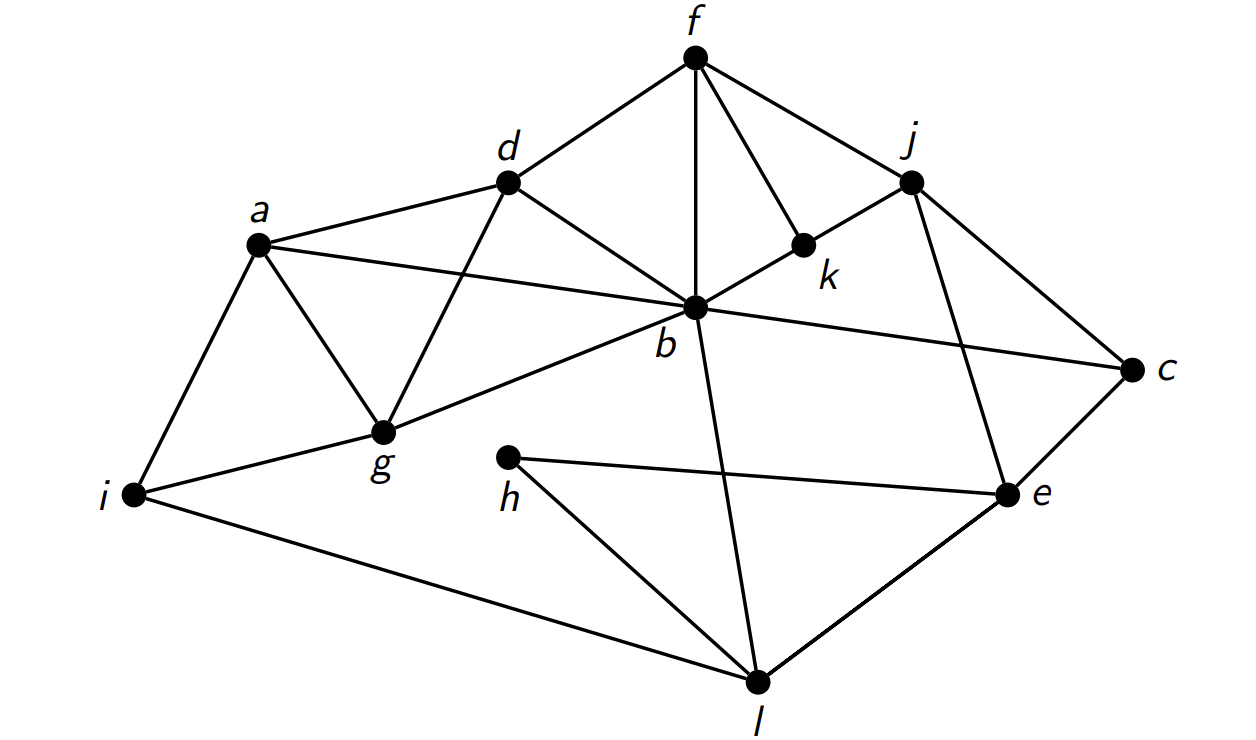
\includegraphics[width=0.56\textwidth]{graph.png}
    \end{center}
    List the corresponding vertices or edges of $G$ for the following:
    \begin{itemize}
        \item Find a clique of size 4/ size 5 if possible
        \item Find a induced cycle of size 4 / size 5 if possible
        \item Find a maximal matching that is \textbf{NOT} maximum.
    \end{itemize}
\end{frame}
\section{Bipartation \& Matching}
\begin{frame}{Bipartation \& Matching}
    \mydef{Theorem}
    For every graph $G$, the following are equivalent:
    \begin{itemize}
        \item $G$ is bipartite
        \item $G$ has no cyle of odd length
        \item $G$ has no closed walk of odd length
        \item $G$ has no induced cycle of odd length.
    \end{itemize}
    \vv 
    \mydef{Compare and Contrast}
    \begin{itemize}
        \item Maximal chain/ maximum chain
        \item Maximal matching/maximum matching
    \end{itemize}
    \yellow{Group Tran ,Transversals?}
    \\ \hh \green{That's difficult QAQ, and let's look at what 
    xrz left us.}
\end{frame}
\begin{frame}
    \frametitle{Hall's Theorem}
    \hh Let $G$ be a bipartite graph with bipartation $\(A, B\)$. There exists a
    matching covering $A$ if\mbox{f} there does not exist $X \subset A$ with $|N\(X\)| < |X|$.
    \\ \vv
    \green{Exercise}
    \\ \hh  Given a sequence of (not necessarily
    distinct) sets $S_1, S_2, \dots, S_m$, there exists a sequence of distinct elements $x_1, x_2, \dots, x_m$ such that
    $x_i ∈ S_i$
    for all $i = 1, 2, \dots, m$ if and only if \textbf{Hall's condition} holds. 
    State \textbf{Hall's condition} in this context.
    \\ \vv
    \pause
    \mysol
        \hh For every $k=1,2,\dots,m$, the union of 
        any $k$ sets has at least $k$ elements, that is 
        $$|\bigcup_{i\in I} S_i|\geq |I\,| \text{ for all } I \subset \{1,\dots,m\}$$
\end{frame}

\section{Algorithms}
\begin{frame}
    \frametitle{Trees}
    Recall them:
    \begin{itemize}
        \item forest
        \item tree 
        \item leaf 
        \item root 
        \item spanning tree
    \end{itemize}
    \begin{block}{Exercise}
        \hh Let $T$ be a tree, $v$ be its leaf. 
        Judge whether the following statements are correct or not :
        \begin{enumerate}
            \item $\comp{G} = |V\(G\)| - |E\(G\)|$
            \item $|V\(T\)|=|E\(T\)|+1$
            \item $T-v$ is a tree
        \end{enumerate}
    \end{block}
\end{frame}
\begin{frame}
    \frametitle{Kruskal's Algorithm}
    \red{Goal:} Find the minimum spanning tree (path of length $n-1$).
    \\ \vv 
    \blue{Steps:}
    \begin{enumerate}
        \item sort the edges according to their costs 
        \item choose the minimum one, that is not choosed yet 
        and would \textbf{not form a cycle}
    \end{enumerate}
    \green{Comment:}\\
        \hh This is a \textit{Greedy Algorithm}. But why is it correct?
\end{frame}
\begin{frame}
    \frametitle{Dijkstra's Algorithm}
    \red{Goal:} Find the minimum distance from the root (one specified vertex).
    \\ \vv 
    
    \blue{Steps:}
    \begin{enumerate}
        \item start from the nearest points you know.
        \item update the distance of other vertexes according to this vertex that you choose.
    \end{enumerate}
    \green{Comment:}\\
        \hh There're other shortest path algorithm, including Freud's Algorithm, Bellman-Ford's Algorithm.
    I guess this would be taught in VE477 by Mn.
    \\ \hh Here is just an overview:
    \\ \hh  \hh \url{https://www.cnblogs.com/fxzemmm/p/14847987.html}
\end{frame}
\section{*Extra Topic}
\begin{frame}
    \frametitle{A Question}
    \hh Wait a moment, there is a question when you apply the Kruskal's 
    Algorithm:

    \begin{center}
        \red{\large{How to judge that, when you are adding 
        one specified edge, would it form a cycle or not? How 
        do computers do that?}}
    \end{center}
    \vs{2em}
    \hh We need a data structure, called \textbf{union and find set}.
\end{frame}
\begin{frame}
    \frametitle{Union and Find Set}
    MAKE\_SET($x$): 
    \begin{center}
        Father [ $x$ ] $\larrow x$ 
    \end{center}
    FIND($x$): \green{Is the father of $x$ itself?}
    \begin{center}
        IF Father [ $x$ ] = x , RETURN $x$.\\
        ELSE RETURN FIND(Father[ $x$ ])
    \end{center}
    UNION($x$,$y$):
    \begin{center}
        Father[ FD$(y)$ ] $\larrow $ FD($x$)
    \end{center}
\end{frame}
\definecolor{mygreen}{rgb}{0,0.6,0}
\definecolor{mygray}{rgb}{0.5,0.5,0.5}
\definecolor{mymauve}{rgb}{0.58,0,0.82}
\definecolor{mypurple}{rgb}{0.58,0.02,0.82}
\definecolor{myblue}{rgb}{0.1,0.2,0.9}
\definecolor{myorange}{rgb}{0.73,0.38,0.17}
\lstset{%
	language=C++,
	backgroundcolor=\color{white},
	basicstyle=\tiny,
	breakatwhitespace=false,
	breaklines=true,
	captionpos=t,
	commentstyle=\color{mygreen},
	deletekeywords={...},
	escapeinside={\%*}{*)},
	extendedchars=true,
	frame=single,
	keepspaces=true,
	keywordstyle=\color{blue},
	%language=Octave,
	%otherkeywords={*,...},
	numbers=left,
	numbersep=5pt,
	numberstyle=\tiny\color{mygray},
	rulecolor=\color{black},
	showspaces=false,
	showstringspaces=false,
	showtabs=false,
	stepnumber=1,
	stringstyle=\color{mymauve},
	tabsize=4,
	title=\lstname
}

\lstdefinestyle{customcpp}{
	belowcaptionskip=0pt,
	breaklines=true,
	%frame=L,
	%xleftmargin=\parindent,
	language=C++,
	showstringspaces=false,
	basicstyle=\scriptsize\ttfamily,
	keywordstyle=\bfseries\color{mypurple},
	commentstyle=\itshape\color{green!40!black},
	identifierstyle=\color{myblue},
	stringstyle=\color{myorange},
}

\lstset{escapechar=@,style=customcpp}
\begin{frame}[fragile]
    \frametitle{A typical Question}
    Question link: \url{https://vijos.org/p/1034}
    \hbox{
    \begin{lstlisting}
    #include <iostream>
    using namespace std;
    int find_root(int* father,int son){
        while (son!=father[son]) son=father[son];
        return son;
    }
    
    int main(){
        int m,n,p;//n people; m relations; enquiry p pairs
        cin >> n >> m >> p;
        int* father=new int[n+1];
        for (int i = 0; i < n; i++){
            father[i+1]=i+1;
        }
        int temp1,temp2;
        int f1,f2;//temperary father\end{lstlisting}
    }
\end{frame}
\begin{frame}[fragile]
    \frametitle{Sample Code(Cont.)}
    \hbox{
    \begin{lstlisting}
        for (int i = 0; i < m; i++){
            cin >> temp1 >> temp2;
            f1=find_root(father,temp1);f2=find_root(father,temp2);
            if (f1!=f2) father[f2]=f1;
        }
        for (int i = 0; i < p; i++){ 
            cin >> temp1 >> temp2;
            f1=find_root(father,temp1);f2=find_root(father,temp2);
            if (f1==f2) cout << "Yes" << endl;
            else cout << "No" << endl;
        }
        delete[] father;
        return 0;
    }\end{lstlisting}
    }
    

\end{frame}
\begin{frame}
    \frametitle{Reference}
    \begin{itemize}
        \item Exercises from Ve203-2020-Fall Assignment.
        \item Exercises from Ve203-2021-Fall TA Xue Runze.
        \item Exericses from Ve203-2021-Summer Final Exam.
        \item Liu Dayou etc.\textit{Data Structure}, third edtion,
        Beijing: Higher Education Press, 2019.5 print.
        %\item Exercises from 2019-Fall-Ve203 TA Yan Xinyu.
        %\item Contents from 2021-Fall Mid\_2\_RC by Xue Runze.
        %\item Yan Shijian, etc. \textit{Basic Number Theory},
        %fourth edition. Beijing: Higher Education Press, 2020.5 print.
    \end{itemize}
\end{frame}
\end{document}